\documentclass[11pt, a4paper]{scrartcl}
\usepackage[utf8]{inputenc}
\usepackage[ngerman]{babel}
\usepackage[T1]{fontenc}
\usepackage{soul}
\usepackage[dvipsnames]{xcolor}
\usepackage{amsmath}
\usepackage{amssymb}
\usepackage{enumitem}
\usepackage{graphicx}
\graphicspath{{images/}}
\usepackage{tikz}
\usetikzlibrary{automata, positioning}


\newcommand{\gr}[1]{{\color{Green}#1}}
\newcommand{\bl}[1]{{\color{RoyalBlue}#1}}
\newcommand{\rd}[1]{{\color{Red}#1}}


\title{Theoretische Informatik}
\author{Zusammenfassung}
\date{SoSe2024}

\begin{document}
\maketitle

\tableofcontents
\newpage


% --- START DES EIGENTLICHEN INHALTS -------------------------------------------------

\section{Allgemein}

\vspace{0.5em}

\subsection{Alphabete und W"orter}

\begin{itemize}
    \item Ein Alphabet $\Sigma$ ist eine endliche Menge unterscheidbarer Symbole
    \item Element $\sigma \in \Sigma$ ist ein Zeichen des Alphabets $\Sigma$
    \item Jedes Element $\omega \in \Sigma^*$  ist ein Wort "uber $\Sigma$
    \item $\varepsilon$ = Leeres Wort
    \item $\Sigma^*$: Menge aller W"orter "uber $\Sigma$
    \item $\Sigma^+$: Menge aller W"orter "uber $\Sigma$ mit mind. 1 Element
    \item $|\omega|$: L"ange eines Wortes ($|\varepsilon|$ = 0)
\end{itemize}

\vspace{1em}

\subsection{Grammatiken}

Eine Grammatik G ist ein 4-Tupel (V, $\Sigma$, P, S):
\begin{itemize}
    \item V: endliche Menge an Nicht-Terminal-Symbolen
    \item $\Sigma$: endliche Menge an Terminal-Symbolen (V$\cap\Sigma=\varnothing$)
    \item P: endliche Menge an Produktionsregeln
    \item S: Startsymbol (S$\in$V)
\end{itemize}

\newpage


\section{Chomsky-Hierarchie}

\vspace{0.5em}

\subsection{Typ 0 ($\mathcal{L}0$) - Phrasenstrukturgrammatiken}

\begin{itemize}
    \item Beliebige Kombination aus T- und NT-Symbolen
\end{itemize}

\vspace{0.5em}

\subsection{ Typ 1 ($\mathcal{L}1$) - Kontextsensitive Grammatiken}

\begin{itemize}
    \item $|l|\leq|r|$
    \item L"ange des Wortes steigt
    \item $S\rightarrow\varepsilon$ erlaubt, wenn S auf \textbf{keiner} rechten Seite einer Regel steht!
\end{itemize}

\raggedright
\textbf{Beispiel:}

$S \rightarrow S'$ | $\varepsilon$ \\
$S' \rightarrow aS'Bc$ | $abc$ \\
$cB \rightarrow Bc$ \\
$bB \rightarrow bb$ 

\vspace{0.5em}

Das Nichtterminal S' braucht man nur, damit die Bedingung der Sonderregel erfüllt ist. 
Das Nichtterminal B wird mal zur Satzform Bc und mal zu bb, je nachdem ob B im \textbf{Kontext} c oder b steht. 

\vspace{0.5em}

\subsection{Typ 2 ($\mathcal{L}2$) - Kontextfreie Grammatiken}

Beim Ableiten in Typ-1-Grammatiken muss man immer aufpassen, dass das Nichtterminal auch im richtigen Kontext steht. 
Das Erzeugen von Sätzen ist viel leichter, wenn die Grammatik kontextfrei ist. 

Eine Grammatik G ist vom Typ 2, wenn sie vom Typ 1 ist und zusätzlich auf der linken Seite jeder Regel genau \textbf{ein} Nichtterminal steht!

\begin{itemize}
    \item $l \in V$
    \item $X \rightarrow \varepsilon$ immer erlaubt
\end{itemize}

\vspace{0.5em}

\subsection{Typ 3 ($\mathcal{L}3$) - Reguläre Grammatik}

Eine Grammatik G ist vom Typ 3, wenn sie vom Typ 2 ist und zusätzlich folgende Regeln hat:

\begin{itemize}
    \item $A \rightarrow b$
    \item $A \rightarrow bC$
    \item $A \rightarrow \varepsilon$
\end{itemize}


\newpage

\section{Deterministischer Endlicher Automat (DEA)}

\hl{Eine DEA M ist ein 5-Tupel (Q, $\Sigma$, $\delta$, $q_0$, F):}

\begin{itemize}
    \item Q: endliche Zustandsmenge
    \item $\Sigma$: endliches Alphabet
    \item $\delta$: $Q \times \Sigma \rightarrow Q$ Übergangsfunktionen
    \item $q_0$: Startzustand
    \item F: Menge der akzeptierten Endzust"ande
\end{itemize}

\vspace{2em}
Beispiel:
\vspace{1em}

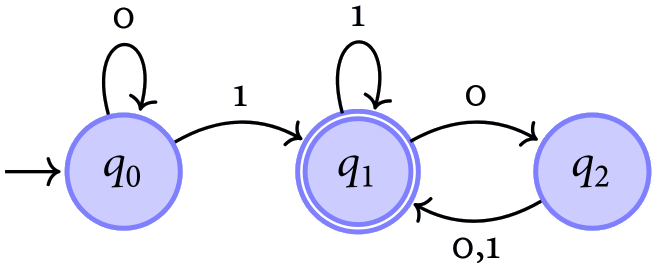
\includegraphics[width=0.4\textwidth]{DEA-00.png}

\begin{itemize}
    \item Q $= \{q_0, q_1, q_2\}$
    \item $\Sigma =$ \{0, 1\}
    \item $q_0 = q_0$
    \item F $= q_2$
    \item $\delta$:
    \begin{itemize}[label={}]
        \item $\delta(q_0, 0) = q_0$
        \item $\delta(q_0, 1) = q_1$
        \item $\delta(q_1, 0) = q_2$
        \item $\delta(q_1, 1) = q_1$
        \item $\delta(q_2, 0) = q_1$
        \item $\delta(q_2, 1) = q_1$
      \end{itemize}
\end{itemize}

\newpage

\section{Nicht-deterministischer Endlicher Automat (NEA)}

\hl{Eine NEA M ist ein 5-Tupel (Q, $\Sigma$, $\delta$, $q_0$, F):}

\begin{itemize}
    \item Q: endliche Zustandsmenge
    \item $\Sigma$: endliches Alphabet
    \item $\delta$: $Q \times \Sigma \rightarrow Q$ Übergangsfunktionen
    \item $q_0$: Menge der Startzust"ande
    \item F: Menge der akzeptierten Endzust"ande
\end{itemize}

\vspace{2em}
Beispiel:
\vspace{1em}

\begin{minipage}[h]{0.45\textwidth}
    $S \rightarrow aS$ | bS | cS | aA \\
    $A \rightarrow bB$ | cC \\
    $B \rightarrow aB$ | bB | cB | $\varepsilon$ \\
    $c \rightarrow aB$
\end{minipage}
\begin{minipage}[h]{0.45\textwidth}
    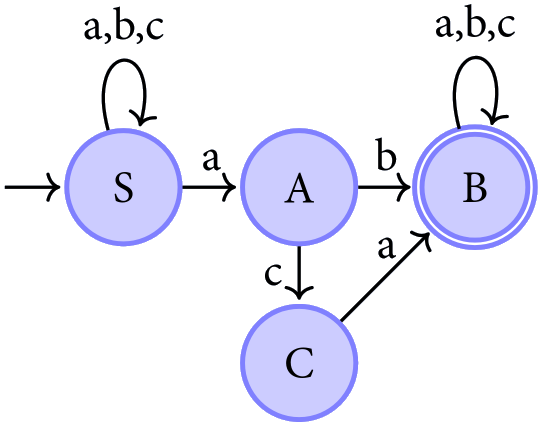
\includegraphics[width=0.7\textwidth]{NEA-00.png}
\end{minipage}

\newpage

\section{Äquivalenz von DEA und NEA}

\subsection{Satz von Rabin und Scott}

Jede von einem NEA akzeptierte Sprache L ist auch von einem DEA akzeptierbar.

\subsection{Potenzmengenkonstruktion (NEA $\rightarrow$ DEA)}

Potezmenge ist die Menge aller Teilmengen



\vspace{2em}

Beispiel:

\vspace{0.5em}

\begin{minipage}[h]{0.40\textwidth}
    \centering 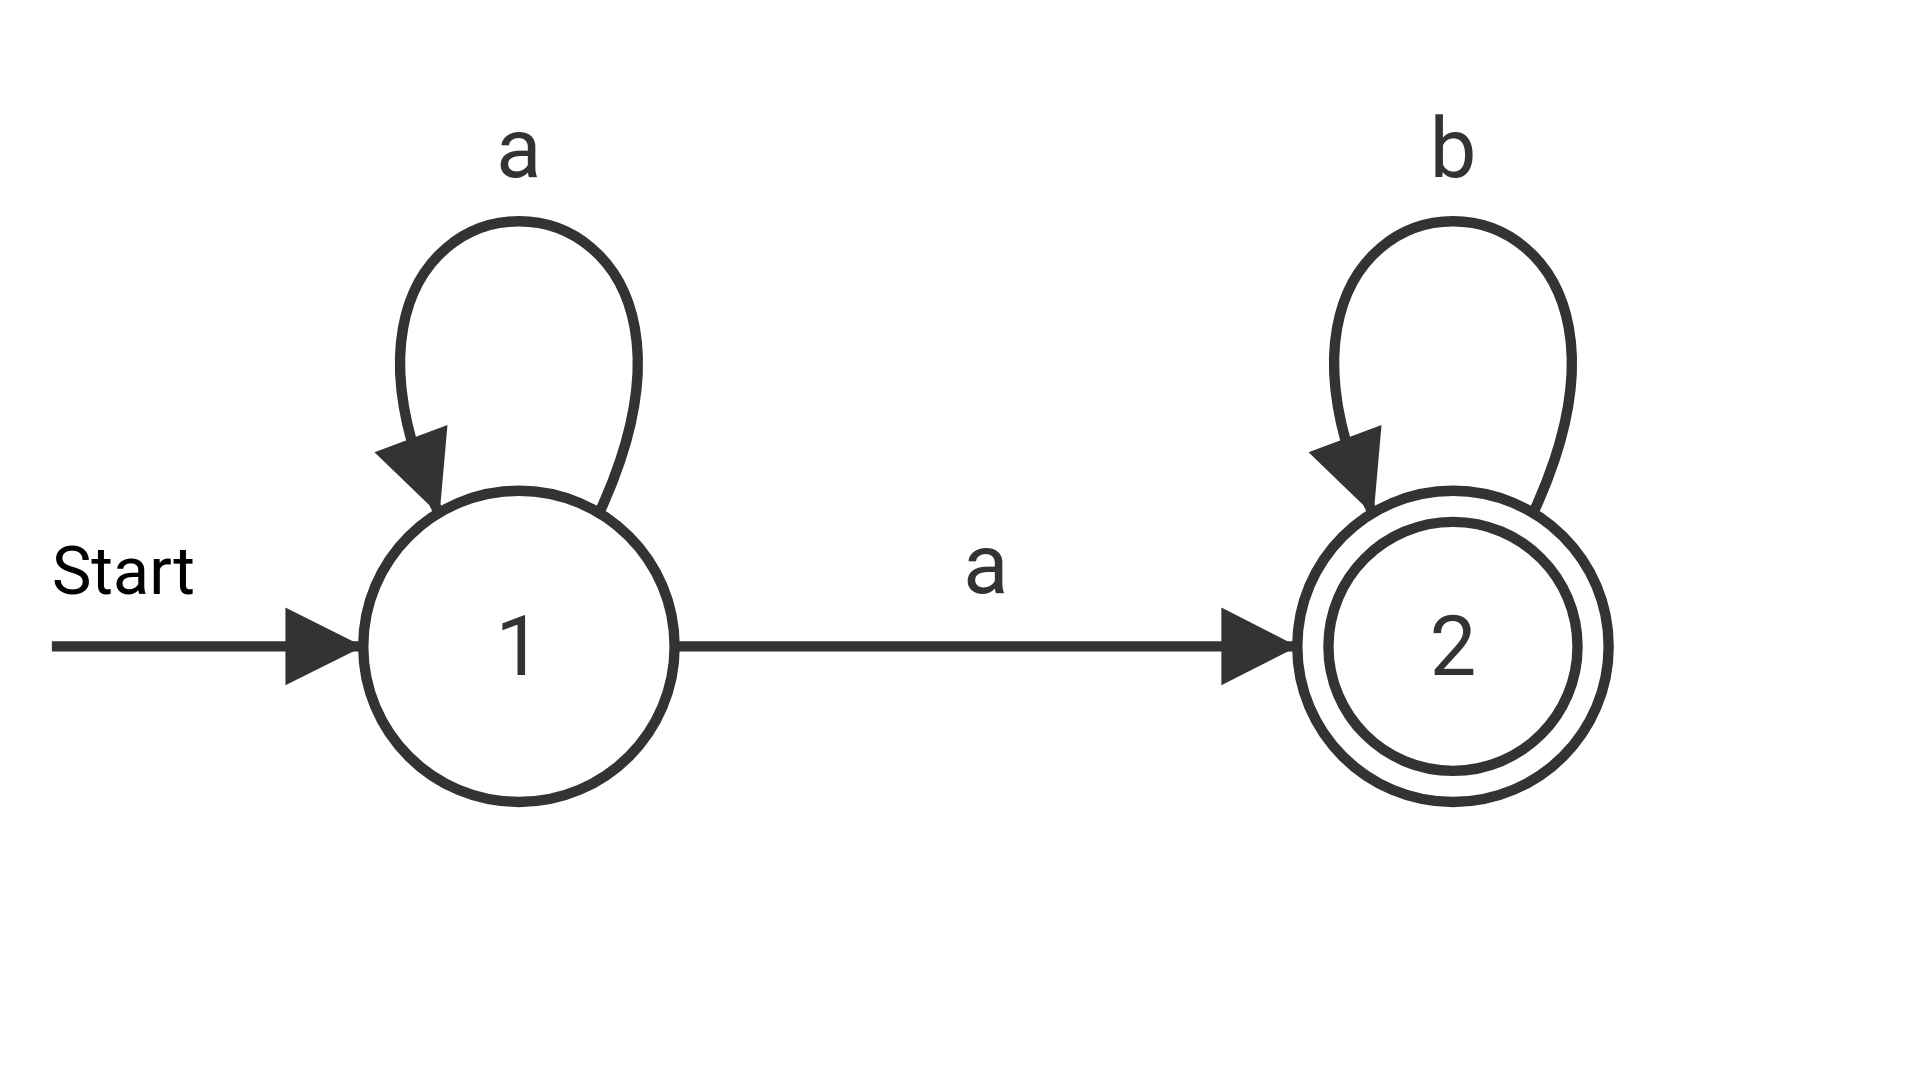
\includegraphics[width=0.75\textwidth]{NEA-01.png}
\end{minipage}
\begin{minipage}[h]{0.10\textwidth}
    \centering $\rightarrow$
\end{minipage}
\begin{minipage}[h]{0.40\textwidth}
    \centering 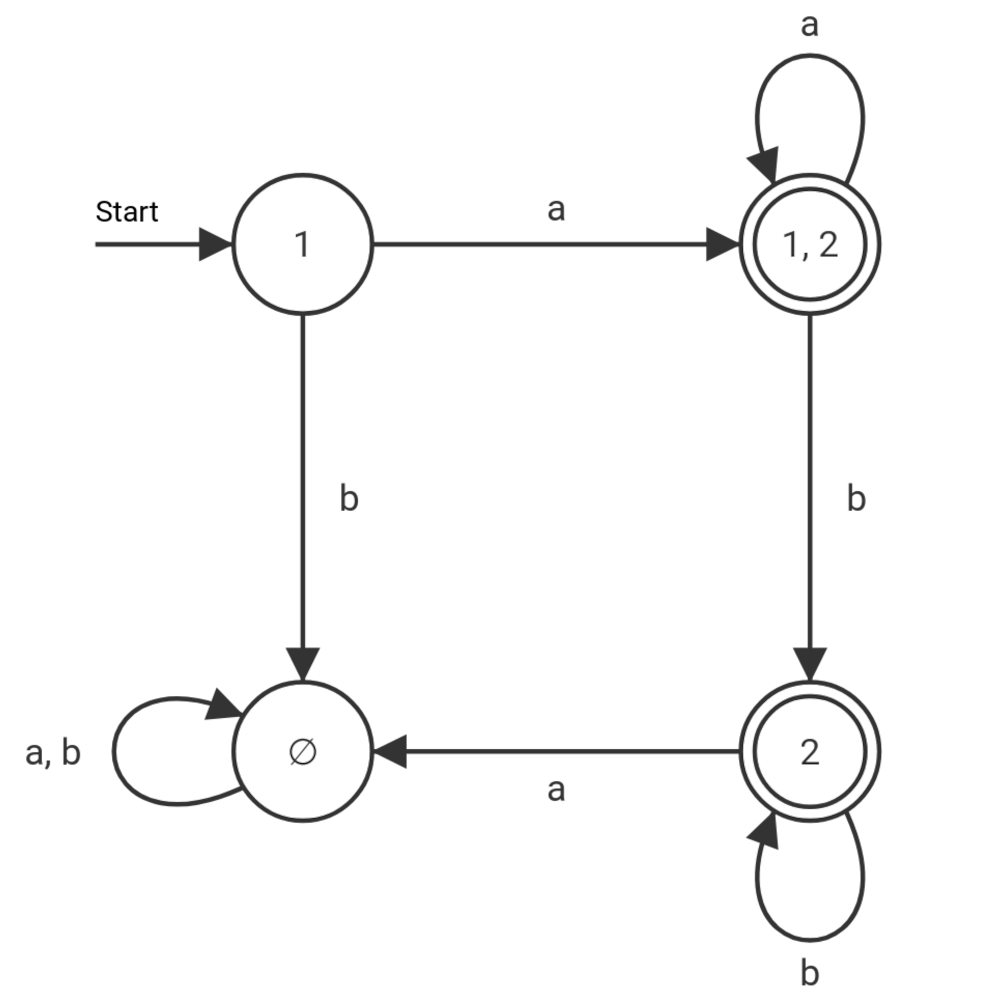
\includegraphics[width=0.85\textwidth]{DEA-01.png}
\end{minipage}

\vspace{0.5em}

\begin{enumerate}
    \item Potenzmenge bilden, $\mathcal{P}\{1, 2\} = \{\{\varnothing \}, \{1\}, \{2\}, \{1, 2\}\}$
    \item Jede Teilmenge ist Zustand des DEA
    \item Wohin kommt man von von jedem NEA Zustand?
    \begin{itemize}
        \item $\delta(\{1\}, a) = 1 \land 2 \rightarrow \{1, 2\}$ 
        \item $\delta(\{1\}, b) = \{\varnothing\}$
        \item $\delta(\{2\}, a) = \{\varnothing\}$
        \item $\delta(\{2\}, b) = \{2\}$
        \item $\delta(\{2\}, b) = \{2\}$
        \item $\delta(\{1, 2\}, a) = \gr{\delta(\{1\}, a)} \cup \rd{\delta(\{2\}, a)} = \gr{1 \land 2} \cup \rd{\varnothing} = \{1, 2\}$
        \item $\delta(\{\varnothing\}, a) \land \delta(\{\varnothing\}, b) = \varnothing \rightarrow \{\varnothing\}$
    \end{itemize}
    \item Startzustand bleibt gleich
    \item Jede Teilmenge, in der der urspr"ungliche Endzustand vorkommt, wird wieder zum Endzustand, $F = 2 \rightarrow F' = \{\{2\}, \{1, 2\}\}$
\end{enumerate}

\newpage


\section{Regex}


\begin{itemize}
    \item \textbf{.} : Beliebiges einzelnes Zeichen außer Zeilenumbruch
    \item \textbf{*} : Null oder mehr Wiederholungen
    \item \textbf{$+$} : Eine oder mehr Wiederholungen
    \item \textbf{\{n\}} : Genau n Wiederholungen
    \item \textbf{\{n,\}} : Mindestens n Wiederholungen
    \item \textbf{\{n, m\}} : Zwischen n und m Wiederholungen
    \item \textbf{[ ]} : Zeichenklasse (z.B. [a-z] für alle Kleinbuchstaben)
    \item \textbf{[ \^\ ]} : Negierte Zeichenklasse
\end{itemize}


Email-Adressen: \verb|[a-zA-Z0-9._%+-]+@[a-zA-Z0-9.-]+\.[a-zA-Z]{2,}|




\subsection{Satz von Kleene}

Die Menge der durch regul"are Ausdr"ucke (Regex) beschreibbaren Sprachen ist genau die Menge der regul"aren Sprachen.

\vspace{0.5em}

$\rightarrow$ Alle endlichen Sprachen sind durch regul"are Ausdr"ucke beschreibbar

\newpage


\section{Pumping Lemma}

%Das Pumping-Lemma wird verwendet, um zu beweisen, dass eine Sprache sicher nicht regul"ar ist.

\begin{itemize}
    \item Wenn L erkennbar ist, dann existiert ein $p \in \mathbb{N}$
    \item sodass f"ur alle W"orter w $\in L$ mit $|w| \geq p$ gilt:
    \item Es gibt eine Zerlegung $w = \rd{x}\gr{y}\bl{z}$ mit $\gr{y} \neq \varepsilon$ und $|\rd{x}\gr{y}| \leq p$,
    \item sodass f"ur alle $i \in \mathbb{N}$ gilt:
    \item $\rd{x}\gr{y^i}\bl{z} \in L$
\end{itemize}

\vspace{2em}

Beispiele:

\vspace{2em}

$L = \{ w \in \{a, b\}^* \quad | \quad |w|_a > |w|_b\}$ 

\vspace{0.5em}

Also eine Sprache, die aus beliebig vielen a und b besteht, aber immer mehr a als b hat.

\vspace{1.5em}

Sei $p \in \mathbb{N}$ gegeben

\vspace{0.5em}

Da unser Wort $|w| \geq p$ sein muss, bietet sich $a^{p+1} b^p$ an.

\vspace{0.5em}

Da $|\rd{x}\gr{y}| \leq p$ gilt, besteht $|\rd{x}\gr{y}|$ also nur aus a.

\vspace{0.5em}

Mit der Zerlegung in $w = \rd{x}\gr{y^i}\bl{z}$ und $i = 0$, h"atte man $|\rd{x}\bl{z}|_a \leq  |\rd{x}\bl{z}|_b$, also weniger a als b.


\vspace{5em}


$L = \{a^{n^2} \quad | \quad n \in \mathbb{N}\}$

\vspace{1.5em}

Sei $p \in \mathbb{N}$ gegeben

\vspace{0.5em}

Da unser Wort $|w| \geq p$ sein muss, bietet sich $w = a^{p^2}$ an.

\vspace{0.5em}

Sei Zerlegung $w = \rd{x}\gr{y^i}\bl{z}$ mit $|\rd{x}\gr{y}| \leq p$ gegeben.

\vspace{0.5em}

Erstes Wort ist $p^2 = |\rd{x}\gr{y}\bl{z}|$

\vspace{0.5em}

N"achst gr"oßere Wort ist $(p+1)^2 = p^2 + 2p + 1$

\vspace{0.5em}

Setze i=2, betrachte $\rd{x}\gr{y^2}\bl{z}$:

\vspace{0.5em}

$|\rd{x}\gr{y}\bl{z}| < |\rd{x}\gr{y^2}\bl{z}|$

\vspace{0.5em}

$|\rd{x}\gr{y^2}\bl{z}| = |\rd{x}\gr{y}\bl{z}| + |\gr{y}|$

\qquad \quad $\leq$ $p^2$ \quad + p (Da y nach $|\rd{x}\gr{y}| \leq p$ h"ochsten L"ange p hat)

\vspace{0.5em}

$p^2 + p < p^2 + 2p + 1$

\vspace{0.5em}

Somit $\rd{x}\gr{y^2}\bl{z} \notin L$





\newpage

\section{Satz von Myhill und Nerode}

Eine Sprache L ist genau dann regul"ar, wenn der Index $R_L$ endlich ist!

\newpage


\section{Minimalautomaten}

\subsection{Table-Filling-Algorithmus}

Nur f"ur DEAs!

\begin{enumerate}
    \item Eventuell nicht erreichbare Zust"ande entfernen
    \item Tabelle aus Zust"anden erstellen \{$q$, $q'$\}, $q \neq q'$
    \item Zustandspaar markieren, bei dem immer \textbf{ein} Zustand ein Endzustand ist
    \item Wiederhole solange, bis keine Markierungen mehr dazu kommen
    \begin{itemize}
            \item F"ur jedes unmarkierte Paar \{$q$, $q'$\} und jeden Buchstaben $a \in \Sigma$
            \begin{itemize}
                \item Wenn \{$\delta(q, a)$, $\delta(q', a)$\} markiert ist, dann das Paar \{$q$, $q'$\} selbst markieren
            \end{itemize}
    \end{itemize}
    \item Verschmelze unmarkierte Zustandspaare
\end{enumerate}

\vspace{3em}

Beispiel Tabelle \{$q$, $q'$\}, $q \neq q'$:

\vspace{0.5em}

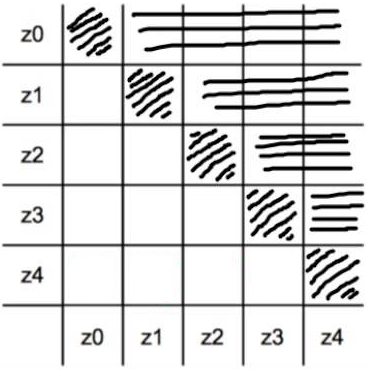
\includegraphics[width=0.4\textwidth]{Minimal-00.png}


\newpage


\section{Kontextfreie Sprachen ($\mathcal{L}2 $)}

\subsection{Chomsky Normalform (CNF)}

Regeln m"ussen folgende Formen haben:

\begin{itemize}
    \item $A \rightarrow BC$
    \item $A \rightarrow a$
    \item $S \rightarrow \varepsilon$
\end{itemize}

\subsection{Greibach Normalform}

Eine $\varepsilon$-freie, kontextfrei Grammatik mit folgenden Regeln:

\begin{itemize}
    \item $A \rightarrow aB_1B_2B_3...B_k$
    \item $k \geq 0$
\end{itemize}

\subsection{Konvertierung}

!!!TODO!!!

\newpage


\section{Kellerautomaten}

\hl{Ein Kellerautomat (PDA) M ist ein 6-Tupel (Q, $\Sigma$, $\Gamma$, $\delta$, $q_0$, $\#$):}

\begin{itemize}
    \item Q: endliche Zustandsmenge
    \item $\Sigma$: endliches Bandalphabet
    \item $\Gamma$: endliches Kelleralphabet
    \item $\delta$: "Ubergansfunktionen
    \item $q_0$: Startzustand ($q_0 \in Q$)
    \item $\#$: "Urspr"ungliches Kellersymbol ($q_0 \in \Gamma$)
\end{itemize}

%Es gibt keinen expliziten Endzustand. Das Ende ist erreicht, wenn auf dem Stack kein Element mehr liegt, oder das Wort komplett gelesen wurde.

\vspace{1em}

Akzeptanz:
\begin{itemize}
    \item Kein akzeptierender Endzustand!
    \item Akzeptanzkriterien für W"orter $x \in |Sigma^*$:
    \begin{enumerate}
        \item Wort komplett gelesen
        \item Keller (Stack leer)
    \end{enumerate}
\end{itemize}

\vspace{1em}

Nicht-Determinismus:
\begin{itemize}
    \item Mehrere simultane "Uberg"ange m"oglich
    \item Spontane "Uberg"ange ($a = \varepsilon$) m"oglich
\end{itemize}

\vspace{1em}

Konfiguration eines PDA gegeben durch 3-Tupel ($Q$, $\Sigma^*$, $\Gamma^*$):
\begin{itemize}
    \item $q \in Q$: Momentaner Zustand
    \item $w' \in \Sigma^*$: Noch zu lesender Anteil der Eingabe
    \item $\gamma \in \Gamma^*$: Aktueller Kellerinhalt
\end{itemize}

\vspace{1em}

"Ubergansfunktion:
\begin{itemize}
    \item $\delta$(q, a, A) $\ni$ ($q', B_1B_2...B_k$)
    \item Wenn Automat in Zustand q ist, das Symbol a liest und A oben auf Stack liegt, wechselt er in Zustand $q'$ und ersetzt das A auf dem Stack durch $B_1B_2...B_k$
\end{itemize}

\newpage



\section{CYK-Algorithmus}

Beispiel:

\begin{itemize}
    \item S $\rightarrow$ ST | TU | US
    \item T $\rightarrow$ SS | a
    \item U $\rightarrow$ TT | b
\end{itemize}

Wort: \textbf{aabab}

\vspace{2em}

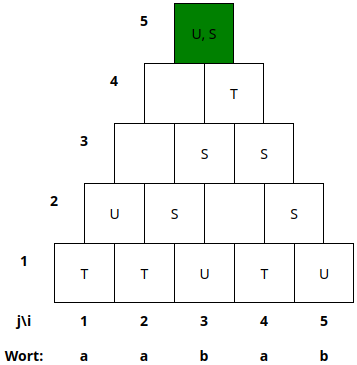
\includegraphics[width=0.5\textwidth]{CYK-00.png}

\vspace{2em}

Nur wenn S (Startsymbol) ganz oben in der Pyramide steht, wird das Wort akzeptiert!

\newpage


\section{Turing-Maschine}

\hl{Eine Turing-Maschine M ist ein 7-Tupel (Q, $\Sigma$, $\Gamma$, $\delta$, $q_0$, $\Box$, F):}

\begin{itemize}
    \item Q: endliche Zustandsmenge
    \item $\Sigma$: endliches Eingabealphabet
    \item $\Gamma$: endliches Arbeitsalphabet ($\Sigma \subset \Gamma$)
    \item $\delta$: "Ubergansfunktionen
    \item $q_0$: Startzustand ($q_0 \in Q$)
    \item $\Box$: Blank-Symbol ($\Box \in \Gamma - \Sigma$)
    \item F: Menge der Endzust"ande
\end{itemize}

\vspace{1em}

"Ubergansfunktionen:
\begin{itemize}
    \item Deterministisch: \qquad \qquad $\delta(q, a) = \delta(q', b, x)$
    \begin{enumerate}
        \item M befindet sich in Zustand $q$ und liest $a$ vom Band
        \item M geht in Zustand $q'$ "uber und ersetzt das $a$ mit einem $b$
        \item M f"uhrt Kopfbewegung $x \in \{l, n, r\}$
      \end{enumerate}

    \item Nicht-deterministisch:\qquad$\delta(q, a) \ni \delta(q', b, x)$
\end{itemize}

\vspace{1em}

Konfiguration einer TM is ein Wort $k \in \Gamma^* Q \Gamma^*$:

$k = \alpha q \beta$\\
$k = \alpha_1...\alpha_m q \beta_1...\beta_n$

\begin{itemize}
    \item $q$: Aktueller Zustand
    \item $\alpha$: Wort links des Schreib/Lese-Kopfes
    \item $\beta$: Wort rechts des Kopfes
\end{itemize}

\vspace{1em}

Startkonfiguration $q_0\vec{w}$:

\begin{itemize}
    \item $w \in \Sigma^*$ steht auf Band
    \item M in Zustand $q_0$
    \item S/L-Kopf steht auf erstem Buchstaben von $w$
    \item Restliches Band mit Blanks $\Box$ bef"ullt
\end{itemize}

\subsection{Linear beschr"ankte Turing-Maschine}

Eine Turing Maschine M ist linear beschr"ankt, wenn $|\vec{w}| < \infty$, also endlich ist.

\section{Satz von Kuroda}

Die von linear beschränkten, nicht-deterministischen Turing-Maschinen akzeptierbaren Sprachen sind genau die kontextsensitiven Sprachen $\mathcal{L}1$




\end{document}